\documentclass[11pt,a4 paper]{article}
\usepackage{amsmath, amsthm} 
\usepackage[english]{babel}
\usepackage[T1]{fontenc}
\usepackage[utf8]{inputenc}
\usepackage[margin=2cm]{geometry}
\usepackage{graphicx}
\usepackage{subfigure}
\usepackage{caption}
\usepackage{siunitx}
\captionsetup{tableposition=top,font=small,width=0.8\textwidth}
\usepackage{booktabs}
\usepackage[table]{xcolor}
\usepackage[arrowdel]{physics}
\usepackage{mathtools}
\usepackage{tablefootnote}
\usepackage{amssymb}
\usepackage{enumitem}
\usepackage{multicol}
\setlist[description]{font={\scshape}} %style=unboxed,style=nextline
\usepackage{wrapfig}
\usepackage{float}
\usepackage{floatflt}
\usepackage{commath}
\usepackage{bm}
\usepackage{nicefrac}
\usepackage{ifthen}
\usepackage{comment}
\usepackage[colorinlistoftodos,textsize=tiny]{todonotes}

\renewcommand*{\thefootnote}{\fnsymbol{footnote}}
\sisetup{exponent-product = \cdot}
\newcommand{\tc}{\,\mbox{tc}\,}
\newcommand{\Epsilon}{\mathcal{E}}
\newcommand{\half}{\frac{1}{2}}
\newcommand{\overbar}[1]{\mkern 1.5mu\overline{\mkern-1.5mu#1\mkern-1.5mu}\mkern 1.5mu}
\let\oldfrac\frac
\renewcommand{\frac}[3][d]{\ifthenelse{\equal{#1}{d}}{\oldfrac{#2}{#3}}{\nicefrac{#2}{#3}}}

\title{Positronium}
\author{Andrea Grossutti, mat. 1237344\\Alessandro Lovo, mat. 1236048\\Leonardo Zampieri, mat. 1237351}
\date{\today}

\begin{document}

\maketitle

\section{Aims}
\begin{itemize}
    \item Measure the ratio between the two and three photons decay of the Positronium;
    \item Measure the lifetime of the Positronium through the time distribution of the decays.
\end{itemize}

\section{Experimental setup}
The experimental setup consist in 4 inorganic scintillators; three coplanar (DET. 1,2,3) and a fourth (DET. 4) perpendicular to the plane.

The first three detector are placed on a circumference in the center of which lies a Na22 source, with an activity of around $380\si{kBq}$. These detector are free movable around the circumference; in this session, two different configurations have been explored. To observe the two-photons decay, the detectors \#1 and \#2 have been aligned; instead, to observe the three-photons decay, the three coplanar detectors have been positioned to form an equilateral triangle.

Data are collected from the detectors through a electronic chain: a fan-in-fan-out quad module reply the signal of each detectors and produce four copies of it; then, through a CFD, a trigger signal is produced.  The CFD trigger threshold has been set so that the background noise is discarded, while the interesting signals produce an output. As can be seen from fig. \ref{fig:oscilloscope}, the signals corresponding to the detection of the $511\si{\kilo\electronvolt}$ and $1275\si{\kilo\electronvolt}$ photons are clearly visible.

\begin{figure}[H]
    \centering
    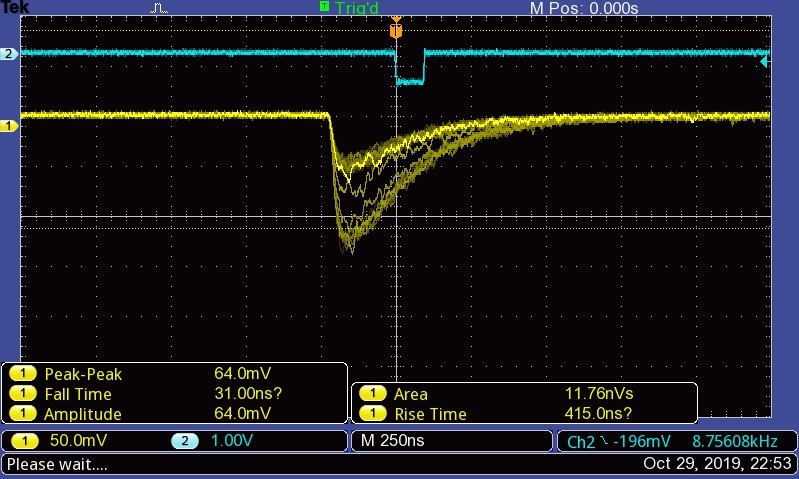
\includegraphics[width=0.7\textwidth]{img/TEK0001.JPG}
    \caption{Signal from the detector (yellow), triggering through the CFD (blu). The two different types of peaks, respectively for the $511\si{\kilo\electronvolt}$ and $1275\si{\kilo\electronvolt}$ photons, are clearly visible. Det. \#2.}
    \label{fig:oscilloscope}
\end{figure}

Between the second and the first day, a technical problem required the substitution of the high voltage power supply; due to this, thresholds have been re-set. While in the first two days all the detectors saw the two peaks around an amplitude of respectively $100$ and $250\si{\milli\volt}$ (and therefore the threshold has been set at about $75\si{\milli\volt}$), in the third day the detectors \#1 and \#3 saw the two peaks around an amplitude of respectively $50$ and $125\si{\milli\volt}$ (and therefore the threshold has been set at about $35\si{\milli\volt}$). For the detector \#4, finally, the threshold has been set to about $200\si{\milli\volt}$, such that only the higher energetic photons produce a trigger.

The CFT is provided of two sets of microswitches, to adjust delay and switch of the output signal. As has been verified thanks to the oscilloscope, the delay microswitches lead  

\end{document}
